% ------------------------------------------------------------------------
% ------------------------------------------------------------------------
% CHRISTIANO VÁRADY	
% Dissertação de Mestrado feita utilizando o modelo de trabalho acadêmico
% da abntex2.
% ------------------------------------------------------------------------
% ------------------------------------------------------------------------

\documentclass[
	% -- opções da classe memoir --
	12pt,				% tamanho da fonte
	%openright,			% capítulos começam em pág ímpar (insere página vazia caso preciso)
	oneside,			% para impressão em verso e anverso. Oposto a oneside
	a4paper,			% tamanho do papel. 
	% -- opções da classe abntex2 --
	sumario=abnt-6027-2012, %sumario todo alinhado a esquerda: abnt-6027-2012 ; sumario mais bonitinho: tradicional
	chapter=TITLE,		% títulos de capítulos convertidos em letras maiúsculas
	%section=TITLE,		% títulos de seções convertidos em letras maiúsculas
	%subsection=TITLE,	% títulos de subseções convertidos em letras maiúsculas
	%subsubsection=TITLE,% títulos de subseções convertidos em letras maiúsculas
	% -- opções do pacote babel --
	english,			% idioma adicional para hifenização
	french,				% idioma adicional para hifenização
	spanish,			% idioma adicional para hifenização
	brazil,				% o último idioma é o prinicipal do documento
	]{abntex2}

% ---
% PACOTES
% ---

% ---
% Pacotes fundamentais 
% ---
\usepackage{cmap}				% Mapear caracteres especiais no PDF
\usepackage{times}				% Usa a fonte Times New Roman
%\usepackage{lmodern}			% Usa a fonte Latin Modern	
\usepackage[T1]{fontenc}		% Selecao de codigos de fonte.
\usepackage[utf8]{inputenc}		% Codificacao do documento (conversão automática dos acentos)
\usepackage{lastpage}			% Usado pela Ficha catalográfica
\usepackage{indentfirst}		% Indenta o primeiro parágrafo de cada seção.
\usepackage{xcolor}				% Controle das cores
\usepackage{graphicx}			% Inclusão de gráficos

%Pacotes adicionados por mim
\usepackage{amsmath}
\usepackage{float}
\usepackage{colortbl}
%\usepackage[table]{xcolor}
\definecolor{lgray}{gray}{0.8}
\usepackage{multirow}
\usepackage{hhline}
\usepackage[scientific-notation=true,round-precision=4]{siunitx}
\newcommand{\mywork}{elaborada pelo autor.}
%Configuracao das legendas de figuras e tabelas1
\usepackage[labelsep=endash,font=small]{caption}
\usepackage{pdfpages}
\usepackage{caption}
\usepackage{subcaption}
\usepackage[section]{placeins}
\usepackage{bm}

% ---
% Pacotes de citações
% ---
%\usepackage[brazilian,hyperpageref]{backref}	 	% Paginas com as citações na bibl
%\usepackage[alf,abnt-etal-cite=2]{abntex2cite}		% Citações padrão ABNT
\usepackage[alf,abnt-etal-list=3,abnt-etal-cite=3]{abntex2cite}  % Citações padrão ABNT

% --- 
% CONFIGURAÇÕES DE PACOTES
% --- 

%% ---
%% Configurações do pacote backref
%% Usado sem a opção hyperpageref de backref
%\renewcommand{\backrefpagesname}{Citado na(s) página(s):~}
%% Texto padrão antes do número das páginas
%\renewcommand{\backref}{}
%% Define os textos da citação
%\renewcommand*{\backrefalt}[4]{
%	\ifcase #1 %
%		Nenhuma citação no texto.%
%	\or
%		Citado na página #2.%
%	\else
%		Citado #1 vezes nas páginas #2.%
%	\fi}%
%% ---


% ---
% Informações de dados para CAPA e FOLHA DE ROSTO
% ---
\titulo{UM AMBIENTE COMPUTACIONAL DE ALTO DESEMPENHO PARA CÁLCULO DE DESLOCAMENTOS USANDO CORRELAÇÃO DE IMAGENS DIGITAIS}
\autor{CHRISTIANO AUGUSTO FERRARIO VÁRADY FILHO}
\local{MACEIÓ/AL}
\data{2016}
\orientador{Prof. Dr. William Wagner Matos Lira}
\instituicao{%
  UNIVERSIDADE FEDERAL DE ALAGOAS -- UFAL
  \par
  CENTRO DE TECNOLOGIA
  \par
  PROGRAMA DE PÓS-GRADUAÇÃO EM ENGENHARIA CIVIL / ESTRUTURAS}
\tipotrabalho{Dissertação (Mestrado)}
% O preambulo deve conter o tipo do trabalho, o objetivo, 
% o nome da instituição e a área de concentração 
\preambulo{Dissertação apresentada ao Programa de Pós-Graduação em Engenharia Civil da Universidade Federal de Alagoas como requisito para obtenção do título de Mestre em Engenharia Civil na área de concentração em Estruturas.}
% ---


% ---
% Configurações de aparência do PDF final

% alterando o aspecto da cor azul
 \definecolor{blue}{RGB}{41,5,195}

% informações do PDF
\makeatletter
\hypersetup{
     %pagebackref=true,
		pdftitle={\@title}, 
		pdfauthor={\@author},
    	pdfsubject={\imprimirpreambulo},
	    pdfcreator={LaTeX with abnTeX2},
		pdfkeywords={Correlação de Imagens Digitais}{Processamento de Imagens}{Computação de Alto Desempenho}, 
		colorlinks=true,       		% false: boxed links; true: colored links
    	linkcolor=black,          	% color of internal links
    	citecolor=black,        		% color of links to bibliography
    	filecolor=black,      		% color of file links
		urlcolor=black,
		bookmarksdepth=4
}
\makeatother
% --- 

% --- 
% Espaçamentos entre linhas e parágrafos 
% --- 

% O tamanho do parágrafo é dado por:
\setlength{\parindent}{1.3cm}

% Controle do espaçamento entre um parágrafo e outro:
\setlength{\parskip}{0.2cm}  % tente também \onelineskip



% "Adequações" à ABNT
% Margens
\setlrmarginsandblock{3cm}{2cm}{*}
\setulmarginsandblock{3cm}{2cm}{*}
\checkandfixthelayout
% Lista de Figuras ao invés de Lista de Ilustrações
\addto\captionsbrazil{%
	\renewcommand{\listfigurename}{Lista de Figuras}
}
% Fonte 12 nos capítulos
\renewcommand{\ABNTEXchapterfontsize}{\normalfont}
\renewcommand{\ABNTEXsectionfontsize}{\normalfont}
\renewcommand{\ABNTEXsubsectionfontsize}{\normalfont}


% ---
% compila o indice
% ---
%\makeindex
% ---

% ----
% Início do documento
% ----
\begin{document}

% Retira espaço extra obsoleto entre as frases.
\frenchspacing 

% ----------------------------------------------------------
% ELEMENTOS PRÉ-TEXTUAIS
% ----------------------------------------------------------
% \pretextual

% ---
% Capa
% ---
\renewcommand{\imprimircapa}{%
\begin{capa}%
\center
\ABNTEXchapterfont \large
UNIVERSIDADE FEDERAL DE ALAGOAS \\
CENTRO DE TECNOLOGIA \\
PROGRAMA DE PÓS-GRADUAÇÃO EM ENGENHARIA CIVIL \\ 
ESTRUTURAS\\
\vspace*{3cm}
{\ABNTEXchapterfont\imprimirautor}
\vspace*{3cm}
\begin{center}
\ABNTEXchapterfont\bfseries\imprimirtitulo
\end{center}
\vfill
\large\imprimirlocal \\
\large\imprimirdata
\vspace*{1cm}
\end{capa}
}
\imprimircapa

% ---

% ---
% Folha de rosto
% (o * indica que haverá a ficha bibliográfica)
% ---
\makeatletter
\renewcommand{\folhaderostocontent}{
\begin{center}
{\ABNTEXchapterfont\large\imprimirautor}
\vspace*{\fill}\vspace*{\fill}
\begin{center}
\ABNTEXchapterfont\bfseries\Large\imprimirtitulo
\end{center}
\vspace*{\fill}
\abntex@ifnotempty{\imprimirpreambulo}{%
\hspace{.45\textwidth}
\begin{minipage}{.5\textwidth}
\SingleSpacing
\imprimirpreambulo \\
\\
{\imprimirorientadorRotulo~\imprimirorientador\par}
\abntex@ifnotempty{\imprimircoorientador}{%
{\imprimircoorientadorRotulo~\imprimircoorientador}%
}%
\end{minipage}%
\vspace*{\fill}
}%
\vfill
{\large\imprimirlocal} \\
{\large\imprimirdata}
\vspace*{1cm}
\end{center}
}
\makeatother

\imprimirfolhaderosto*
% ---

 \begin{fichacatalografica}
     \includepdf{Fichacat5135-2016.pdf}
 \end{fichacatalografica}
 
\addtocounter{page}{-1}

% ---

 \begin{folhadeaprovacao}
     \includepdf{Faprov.pdf}
 \end{folhadeaprovacao}
 
\addtocounter{page}{-1}


%% ---
%% Agradecimentos
%% ---
\begin{agradecimentos}
 \noindent{A meus pais, por me ensinarem a buscar meus objetivos.}
 
 \noindent{A Paula, por participar comigo de todos os momentos dessa vitória.}
 
 \noindent{Ao professor William Lira, pela orientação em todas as pesquisas.}
 
 \noindent{Ao professor Eduardo Toledo, pelo auxílio nas muitas solicitações que fiz ao PPGEC.}
 
 \noindent{Aos colegas do LCCV Ricardo e Catarina Fernandes, Lucas Gouveia e Tiago Lobo pelo apoio no desenvolvimento do trabalho.}
 
 \noindent{Ao colega Romildo Escarpini, pelas muitas discussões e pelo apoio durante toda a dissertação.}
 
 \noindent{Ao CNPq, pela bolsa dispensada.}
 
\end{agradecimentos}

 \begin{epigrafe}
 	
 	\vspace*{\fill}
 	\begin{flushright}
 		\textit{“The mind itself has no needs, except for those it creates itself. Is undisturbed, except for its own disturbances. Knows no obstructions, except those from within” \\ }
 		\vspace{1cm}
 		\textit{Marcus Aurelius - Meditations}
 	\end{flushright}
 	
 \end{epigrafe}
%% ---

% ---
% RESUMOS
% ---

% resumo em português
\setlength{\absparsep}{18pt} % ajusta o espaçamento dos parágrafos do resumo
\begin{resumo} 
\label{resumo}

O presente trabalho apresenta um ambiente computacional de alto desempenho que utiliza técnicas de correlação de imagens digitais para determinação de grandezas físicas associadas a problemas de engenharia. Sua arquitetura computacional integra diversas tecnologias avançadas para o cálculo dos campos de deslocamentos de elementos estruturais a partir de ensaios. A metodologia utilizada prevê o estudo de conceitos, formulações e técnicas de arquitetura de \textit{software}, processamento de imagens, correlação de imagens digitais e computação de alto desempenho, além de incorporar procedimentos específicos em um ambiente único para a determinação de grandezas físicas. Dentre os principais procedimentos utilizados na arquitetura apresentada, pode-se citar as abordagens locais e globais de correlação de imagens digitais, métodos de otimização não-linear e interpolações bidimensionais. Também são incorporadas ao ambiente computacional estratégias de computação de alto desempenho para alcançar ganhos de performance na determinação dos campos de deslocamentos e deformações usando a correlação de imagens digitais. Uma comparação com o método \textit{Scale Invariant Feature Transform} e com o método Q4-DIC de análise de imagens também são realizadas. Um protótipo computacional é desenvolvido com o objetivo de validar o ambiente de alto desempenho apresentado, permitindo o monitoramento de elementos estruturais através da correlação de imagens digitais. Também são realizados estudos de casos que permitem a verificação de tecnologias incorporadas ao protótipo apresentado, incluindo análises quantitativas de resultados e medição de tempo computacional.

 \textbf{Palavras-chaves}: Correlação de imagens digitais. Processamento de imagens. Computação de alto desempenho.
\end{resumo}


% resumo em inglês
\begin{resumo}[Abstract]
 \begin{otherlanguage*}{english}

This work proposes a high performance computing environment using digital image correlation techniques to determine physical quantities associated with engineering problems. Software architecture supports this computing environment, integrating several advanced technologies for calculation of displacement and strain fields of structural elements from testing. The methodology applies the study of concepts, formulations and techniques for image processing, digital image correlation, high performance computing and software architecture. The methodology also includes specific procedures in a single environment for the evaluation of physical quantities. Among the main procedures used in the presented software architecture, one can cite the digital image correlation techniques known as Full-Field and Subset, non-linear optimization methods and two-dimensional interpolations. In addition, high performance computing strategies are included into the computing environment to achieve performance speed-ups on evaluating the displacement fields using digital image correlation. Comparisons with \textit{Scale Invariant Feature Transform} and Q4-DIC are also evaluated. Following, the development of a computer prototype has the purpose of validating the presented high performance environment, allowing the calculation of physical quantities in structural elements through the correlation of digital images. Then, submission of case studies into the prototype validates data acquired from technologies built into the prototype, including quantitative analysis of results and measurement of computational time.

   \textbf{Keywords}: Digital image correlation. Image processing. High performance computing
 \end{otherlanguage*}
\end{resumo}

% ---
% inserir lista de ilustrações
% ---
\pdfbookmark[0]{\listfigurename}{lof}
\listoffigures*
\cleardoublepage
% ---

% ---
% inserir lista de tabelas
% ---
\pdfbookmark[0]{\listtablename}{lot}
\listoftables*
\cleardoublepage
% ---

%% ---
%% inserir lista de abreviaturas e siglas
%% ---
%\begin{siglas}
%  \item[CID] Correlação de Imagens Digitais
%  \item[HPC] \textit{High Performance Computing} - Computação de Alto Desempenho
%\end{siglas}
%% ---

% ---
% inserir lista de símbolos
% ---
%\begin{simbolos}  

%  \item[$A$] Evento qualquer do domínio $\Omega$
%  \item[$A_c$] Constante empírica na formulação de $R_{o\mathrm{P}}$
%  \item[$\boldsymbol{A}$] Matriz auxiliar para resolução do SORM
%  \item[$\boldsymbol{A}^*$] Matriz auxiliar para resolução do SORM
%  \item[$A_\mathrm{i}$] Área interna do tubo
%  \item[$A_\mathrm{o}$] Área externa do tubo
%  \item[$A_\mathrm{s}$] Área da seção transversal do tubo
%  \item[$a$] Profundidade máxima de uma trinca na parede do tubo devido ao processo de produção

%  
%%%%% SÍMBOLOS GREGOS %%%
%
%  \item[$\boldsymbol{\alpha}$] Vetor unitário com direção e sentido de $\boldsymbol{y}^{\mathrm{d}}$
%  
%  \item[$\beta$] Índice de confiabilidade
%  
%  \item[$\Gamma$] Função Gamma
%
%  \item[$\Delta P$] Diferencial de pressão
%  \item[$\Delta P_{\mathrm{TL}}$] Diferencial de pressão do cenário hipotético de \textit{tubing leak}
%  \item[$\Delta R_{i\mathrm{API}}$] Diferencial de pressão resistente para \citeauthoronline{API5C31994} (pressão interna)
%  \item[$\Delta R_{i\mathrm{KS}}$] Diferencial de pressão resistente com ações combinadas para \citeonline{klever1998analytical} (pressão interna - ruptura dúctil do tubo)
%  \item[$\Delta R_{i\mathrm{KSn}}$] Diferencial de pressão resistente com ações combinadas para \citeonline{klever1998analytical} (pressão interna - empescoçamento do tubo)
%  \item[$\Delta R_{o\mathrm{API}}$] Diferencial de pressão resistente com ações combinadas para \citeauthoronline{API5C31994} (pressão externa)

%\end{simbolos}
% ---


% ---
% inserir o sumario
% ---
\pdfbookmark[0]{\contentsname}{toc}
\tableofcontents*
\cleardoublepage
% ---

% ----------------------------------------------------------
% ELEMENTOS TEXTUAIS
% ----------------------------------------------------------
\textual

\section{INTRODUÇÃO}

%texto \cite{ceccato2021two} oi

texto2 \citeonline{ceccato2021two} oi

\chapter{REVISÃO DE LITERATURA}

\section{Perfuração de Poços de Petróleo}

A perfuração de poços de petróleo constitui uma das etapas mais importantes das operações de exploração e produção, sendo responsável por estabelecer a comunicação entre a superfície e os reservatórios produtores. De modo geral, o poço é perfurado em fases sucessivas, definidas de acordo com as características geológicas das formações atravessadas e com a profundidade prevista do projeto. Ao término de cada fase, realiza-se a descida e cimentação de uma coluna de revestimento, cuja principal função é garantir a estabilidade do poço, prevenir o desmoronamento das formações, controlar a migração de fluidos e assegurar condições adequadas de segurança operacional ao longo da perfuração \cite{thomas2001}.

Dessa forma, a classificação dos revestimentos também possui grande importância no projeto de poços, uma vez que permite diferenciá-los de acordo com a função desempenhada em cada etapa da perfuração. De modo geral, os revestimentos podem ser classificados em condutor, de superfície, intermediário e de produção, conforme ilustrado na Figura \ref{fig:Figura01_revest}.

\begin{figure}[H]
	\centering
	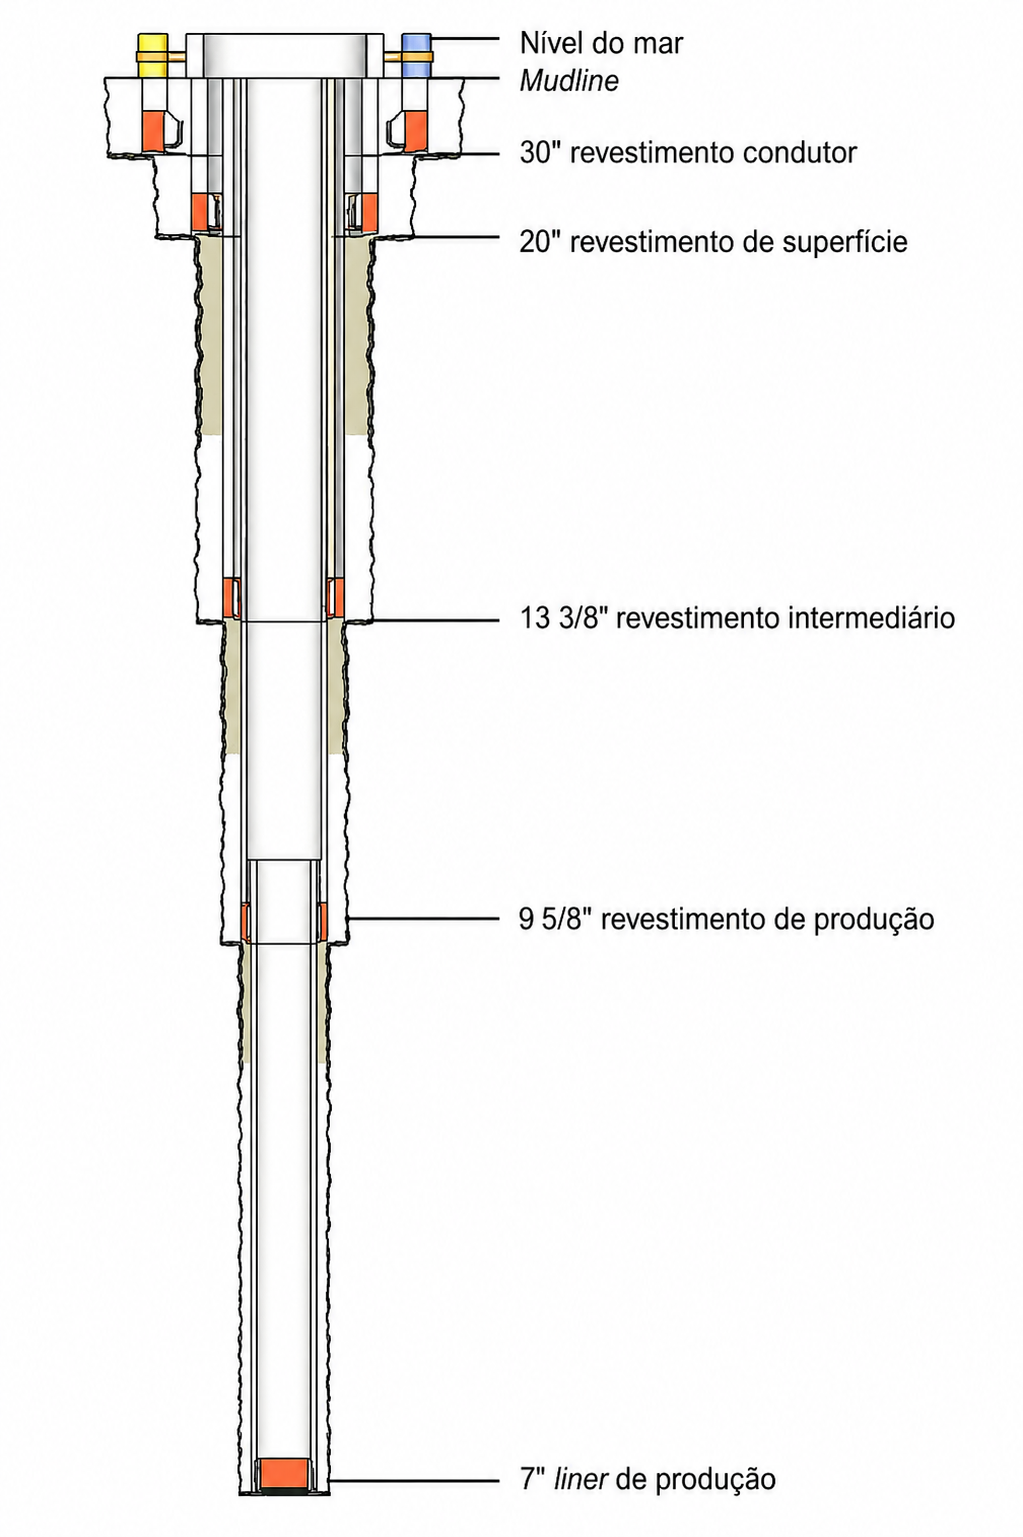
\includegraphics[width=0.5\linewidth]{figuras/Figura1_revest.png}
	\caption{Esquema de revestimento de poços. Fonte: \citeonline{rocha2009}}
	\label{fig:Figura01_revest}
\end{figure}

\citeonline{thomas2001} traz que o revestimento condutor corresponde à primeira coluna instalada no poço, sendo assentado a pequenas profundidades. Sua principal função é sustentar os sedimentos superficiais pouco consolidados, proporcionando estabilidade inicial à perfuração. A instalação desse revestimento pode ser realizada por cravação, jateamento ou perfuração seguida de cimentação, dependendo das condições geotécnicas do local.

O revestimento de superfície é descido após a perfuração das primeiras fases do poço e tem como objetivo proteger formações rasas, evitar o desmoronamento de zonas inconsolidadas e isolar aquíferos próximos à superfície. Além disso, essa coluna também atua como base de apoio para os equipamentos instalados na cabeça do poço e para as colunas subsequentes.

O revestimento intermediário tem como finalidade o isolamento de zonas específicas ao longo da perfuração, como formações instáveis, regiões com perda de circulação ou intervalos submetidos a pressões elevadas. Sequencialmente, o revestimento de produção é instalado na região do reservatório com a finalidade de permitir a produção de óleo e gás, além de garantir o isolamento entre as zonas produtoras e as demais formações atravessadas pelo poço. Em alguns casos, pode ser complementado pela utilização de liners, que correspondem a colunas de revestimento parcialmente ancoradas na coluna anterior.

Após o assentamento do revestimento, realiza-se a cimentação do poço, processo responsável pelo preenchimento do espaço anular entre o revestimento e as paredes da formação, garantindo a fixação da coluna e o isolamento hidráulico entre as zonas atravessadas \cite{rocha2009}. Em seguida, podem ser executadas operações de perfilagem e avaliação da formação, repetindo-se esse ciclo até a conclusão de todas as fases do poço.

\section{Instalação do revestimento condutor}

\subsection{Perfurado e cimentado}

\subsection{Base torpedo}

\subsection{Jateamento}

\subsection{Cravação por martelamento}

\section{Modelos constitutivos}

\section{Mohr-Coulomb}

\subsection{Drucker-Prager}

\subsection{Cam-clay}

\subsection{Norsand}

\section{Método dos Pontos Materiais}

\subsection{Two-phase single point}

\subsection{Algoritmo de contato}

\subsection{Algoritmo de corpo rígido}

\subsection{Malha móvel}

\section{Parâmetros do solo}

\subsection{CPTu}

\section{Estado da arte}

\chapter{METODOLOGIA}

\section{Modelo numérico}

\section{Propriedades dos materiais}

	A definição adequada das propriedades dos materiais e dos parâmetros do modelo constitutivo é essencial para garantir a representatividade das simulações numéricas. Assim, de acordo com os dados de resistência à compressão foi possível classificar o solo como uma argila muito mole, considerando-se o critério adotado por \citet{maragon2008}.

Os dados de ensaio CPTu utilizados são disponibilizados pela operadora, a partir dos quais constatou-se que o modelo constitutivo de Mohr-Coulomb seria adequado para modelar a resposta do solo. A Tabela \ref{tab:propriedades_crav} contém as propriedades dos materiais considerados para modelar o solo coesivo não drenado em questão.

\begin{table}[H]
	\centering
	\footnotesize % Reduz tamanho da fonte
	\renewcommand{\arraystretch}{1.2} % Aumenta espaçamento entre linhas
	\setlength{\tabcolsep}{4pt} % Ajusta espaçamento entre colunas
	\begin{tabular}{|cccccc|}
		\hline
		\multicolumn{1}{|c|}{\multirow{2}{*}{\textbf{Propriedades}}} &
		\multicolumn{4}{c|}{\textbf{Valor}} &
		\multirow{2}{*}{\textbf{Unidade}} \\ \cline{2-5}
		\multicolumn{1}{|c|}{} &
		\multicolumn{1}{c|}{Camda 1} &
		\multicolumn{1}{c|}{Camada 2} &
		\multicolumn{1}{c|}{Camada 3} &
		\multicolumn{1}{c|}{Camada 4} &
		\\ \hline
		\multicolumn{1}{|c|}{\textbf{Classificação}} &
		\multicolumn{1}{c|}{Argila muito mole} &
		\multicolumn{1}{l|}{Argila muito mole} &
		\multicolumn{1}{l|}{Argila mole} &
		\multicolumn{1}{l|}{Argila média} &
		\multicolumn{1}{l|}{} \\ \hline
		\multicolumn{1}{|c|}{\textbf{Porosidade inicial}} &
		\multicolumn{1}{c|}{0.58} &
		\multicolumn{1}{c|}{0.58} &
		\multicolumn{1}{c|}{0.47} &
		\multicolumn{1}{c|}{0.43} &
		- \\ \hline
		\multicolumn{1}{|c|}{\textbf{Densidade}} &
		\multicolumn{1}{c|}{1,475.40} &
		\multicolumn{1}{c|}{1,687.91} &
		\multicolumn{1}{c|}{1,799.32} &
		\multicolumn{1}{c|}{1,838.82} &
		Kg/m³ \\ \hline
		\multicolumn{1}{|c|}{\textbf{Coeficiente de Poisson \linebreak efetivo}} &
		\multicolumn{1}{c|}{0.49} &
		\multicolumn{1}{c|}{0.49} &
		\multicolumn{1}{c|}{0.45} &
		\multicolumn{1}{c|}{0.40} &
		- \\ \hline
		\multicolumn{1}{|c|}{\textbf{Valor de K0}} &
		\multicolumn{1}{c|}{0.96} &
		\multicolumn{1}{c|}{0.96} &
		\multicolumn{1}{c|}{0.82} &
		\multicolumn{1}{c|}{0.67} &
		- \\ \hline
		\multicolumn{1}{|c|}{\textbf{Módulo de elasticidade efetivo}} &
		\multicolumn{1}{c|}{17,896.07} &
		\multicolumn{1}{c|}{27,823.35} &
		\multicolumn{1}{c|}{60,440.32} &
		\multicolumn{1}{c|}{83,865.38} &
		kPa \\ \hline
		\multicolumn{1}{|c|}{\textbf{Coesão efetiva}} &
		\multicolumn{1}{c|}{9,27} &
		\multicolumn{1}{c|}{36.23} &
		\multicolumn{1}{c|}{93.95} &
		\multicolumn{1}{c|}{148.92} &
		kPa \\ \hline
		\multicolumn{1}{|c|}{\textbf{Ângulo de atrito efetivo}} &
		\multicolumn{1}{c|}{36.29} &
		\multicolumn{1}{c|}{37.99} &
		\multicolumn{1}{c|}{40.35} &
		\multicolumn{1}{c|}{37.63} &
		graus \\ \hline
		\multicolumn{1}{|c|}{\textbf{Ângulo de atrito (contato)}} &
		\multicolumn{1}{c|}{0.43} &
		\multicolumn{1}{c|}{0.44} &
		\multicolumn{1}{c|}{0.47} &
		\multicolumn{1}{c|}{0.44} &
		rad \\ \hline
		\multicolumn{1}{|c|}{\textbf{Fator de adesão}} &
		\multicolumn{1}{c|}{4.64} &
		\multicolumn{1}{c|}{18.12} &
		\multicolumn{1}{c|}{46.97} &
		\multicolumn{1}{c|}{74.46} &
		kPa \\ \hline
		\multicolumn{6}{|c|}{\textbf{Água}} \\ \hline
		\multicolumn{1}{|c|}{\textbf{Densidade}} &
		\multicolumn{4}{c|}{1000} &
		Kg/m³ \\ \hline
		\multicolumn{1}{|c|}{\textbf{Permeabilidade intrínseca}} &
		\multicolumn{4}{c|}{1.0214x10-9} &
		m³/s \\ \hline
		\multicolumn{1}{|c|}{\textbf{Módulo volumétrico}} &
		\multicolumn{4}{c|}{2.15x104} &
		kPa \\ \hline
		\multicolumn{1}{|c|}{\textbf{Viscosidade dinâmica}} &
		\multicolumn{4}{c|}{1.5673x10-6} &
		kPa   s \\ \hline
	\end{tabular}
	\caption{Propriedades utilizadas para modelar o solo coesivo não drenado}
	\label{tab:propriedades_crav}
\end{table}

No modelo, o revestimento condutor possui propriedades do aço é considerado como um corpo rígido, com densidade de 7860 kg/m³.   

\include{diss_cap4}

\include{diss_cap5}

% \include{diss_cap6}

\include{diss_cap7}

%\include{diss_sift}

\null
\vfill

\bookmarksetup{startatroot}% 

\postextual


% ----------------------------------------------------------
% Referências bibliográficas
% ----------------------------------------------------------
\bibliography{RevBib}

\end{document}